\documentclass[12pt, oneside]{article}   	% use "amsart" instead of "article" for AMSLaTeX format
\usepackage{geometry}                		% See geometry.pdf to learn the layout options. There are lots.
\geometry{a4paper}                   		% ... or a4paper or a5paper or ... 
%\geometry{landscape}                		% Activate for rotated page geometry
%\usepackage[parfill]{parskip}    		% Activate to begin paragraphs with an empty line rather than an indent
\usepackage{graphicx}				% Use pdf, png, jpg, or eps§ with pdflatex; use eps in DVI mode
								% TeX will automatically convert eps --> pdf in pdflatex		
\usepackage{amssymb}
\usepackage{amsmath}
\usepackage{authblk}
\usepackage[hyphens]{url}

\usepackage{url}
\usepackage{hyperref} 

\usepackage{titlesec}

\usepackage{caption}

\usepackage{float}


\title{A Comprehensive Approach to Ecosystem Services Management: From Alarm to Action}
\author{Aidan T. Parkinson; Andreea M. Benu}

\date{\today}							% Activate to display a given date or no date

\begin{document}
\maketitle
\begin{center}
\href{mailto:enquiries@aidantparkinson.com}{enquiries@aidantparkinson.com}
\end{center}

\section{Abstract}
This paper examines how societies can coordinate fairly when nation-states cannot manage our common ecosystem alone.
It recognises that no society is entirely free from political realities or the costs involved in maintaining social order.
As a result, ideal propositions of social cooperation, such as John Rawls’s The Law of Peoples, remain incomplete when considering practical application.
We introduce the Commonwealth Cost of Carbon, as a new Ecosystem Performance Observation that measures how much societies spend to maintain order relative to their total activity.
This ratio provides a transparent and replicable way to assess global ecosystem performance without relying on specialist expertise or privileged data.
Between 2000 and 2020, this cost increased from approximately $65 to $140 per tonne of CO₂e, suggesting both a decline in ecosystem performance and a rising social value for emission reduction.
Building on this indicator, we propose the Commonwealth of Peoples as a new trade association, that translates moral duty into service quality.
Here, a complementary Service Rating is introduced, serving as a cost–benefit ratio that benchmarks site industrial intensity.
Together, these tools provide a performance-based foundation of ecosystem governance that provides an assured approach to move a society from alarm to action.

\section{Introduction}

We live in an age where global crises such as climate change, biodiversity loss, and geopolitical instability overlap and compete for attention. Yet our tools for cooperation are often inadequate.
Such unrest raises a deeper question: how societies can coordinate fairly when nation-states cannot manage our common ecosystem alone?\\

For centuries, thinkers from Hobbes to Rawls have debated how communities balance self-interest with duty to the wider world.
Their ideas provide language for rethinking today’s governance of our common ecosystem.
John Rawls, for example, argued in The Law of Peoples that \emph{"Peoples have a duty to assist other Peoples living under unfavourable conditions that prevent their having a just or decent political and social regime."}~\cite{jr2}.
Yet in truth, everyone today lives under some form of unfavourable condition as a result of natural limitations in social development.
This implies a shared duty to sustain the systems that make our lives worth living, whatever perspective one takes a genuine interest from to such a diverse and complex issue.
So, is it realistic to imagine an entirely reasonable society unaffected by the imperfect Realpolitik of nation-states?\\

Philosophers describe the \emph{"State of Nature"} as life without shared rules: sometimes cooperative~\cite{jl1}~\cite{rn1}, sometimes chaotic and conflict-ridden~\cite{th1}.
If our global order today resembles such a State, what responsibilities do we still owe one another?
Should these duties fall primarily to nation-states, to individuals, or to organisations?
What can a reasonable person do for the common good, and how might such efforts be organised into a fairer society?
Neither the ideal society Rawls proposes nor the sovereign authority Hobbes demands seems appropriate for today’s ecological and political realities.
We evidently live in a hybrid ecosystem, too pluralist to ever submit to one absolute authority, with many presenting a continual challenge to any shared sense of utopia.\\

This tension suggests that ordinary people and institutions alike share a responsibility not grounded in perfection, but in doing the \emph{"Best We Can"}.
Our argument is that our shared Best We Can society provides the more complete form of social contract that Rawls anticipated, but could not fully realise.
As a result, this paper argues for a new trade association known as the \emph{"Commonwealth of Peoples"}: which is not a utopian ideal, but an agile inter-network with shared interests in sustainable development.
In such a society, all members share a minimal duty of service toward the commons, operationalised through an Ecosystem Performance Observation, specifically, our novel definition of the \emph{"Commonwealth Cost of Carbon"} (CCC).
Where Rawls imagines a perfectly reasonable society of cooperating Peoples, the Commonwealth of Peoples embraces deep-rooted philosophical pluralism and persistent disagreement on pivotal global questions.
This framework exhibits the resilience needed for meaningful action within the constraints of Realpolitik.
It offers a more workable social contract: one in which imperfect actors coordinate fairly by balancing duties to one another with their impact on the wider ecosystem.
It also renews focus on demand-side assurance and advisory for private entities, while maintaining a global perspective.
Over time, the Commonwealth of Peoples has the potential to scale universally across all end-use services.\\

From this point of departure, the research moves from exploring theory to developing practice.
The remainder of this paper discusses the strategic planning necessary to translate philosophy into action.
This exercise is limited to the authors’ combined experience, though serves to illustrate a shared vision for development.
A newly formulated Service Rating is introduced to classify end-use services, drawing upon our novel Ecosystem Performance Observation.
This indicator informs a scenario-planning exercise that defines expectations for a new School of Ecosystem Management.
The paper concludes with a reflective evaluation of the associations achievements and present limitations.\\

\section{Ecosystem Performance Observation}

It is difficult to imagine any society free from the political realities and territorial disputes that shape nation-states.
Even the most reasonable communities must often comply with political decisions they neither designed nor fully endorsed.
These compromises create what economists call ecosystem externalities: resulting in social costs that fall outside formal markets or capital budgets.
For societies to act in the common interest, such externalities need to be recognised and internalised within decision-making~\cite{rc1}.
Therefore, our Ecosystem Performance Observation becomes a necessary instrument of any Best We Can social contract: a way that develops trust, credibility, and continual learning from the State of our common ecosystem.\\

At its core, observing ecosystem performance means examining the consequences of human activity.
Every transaction, service, or agreement produces material and energetic by-products, such as waste, water quality, and greenhouse-gas emissions.
While many forms of waste can be managed locally by territorial authorities, greenhouse gases are different: once released, they enter a common planetary ecosystem.
Emissions anywhere may most affect quite remote conditions.
Further, as carbon-based lifeforms, anthropogenic greenhouse gas emissions have deep rooted dependencies with human activity.
This makes greenhouse gas emissions a particularly strong candidate for a common signal that relates human influence on the State of the global commons.\\

Earth’s carbon sinks, its atmosphere, forests, oceans, and soils, absorb greenhouse gas emissions and support the carbon cycle.
The condition of these sinks is itself a performance indicator: their capacity is pivotal in determining mean surface temperature, which influences conditions of the wider ecosystem.\\
Measuring economic output alone cannot capture this reality.
A society that grows while overloading these sinks cannot be said to perform well.
In order to respond reasonably, one needs to recognise that these productive assets have a crucial relationship with \emph{Enabling Assets}: institutions, knowledge, networks and time.
These human-made Enabling Assets shape social production and observable behaviour and can be envisaged as enabling software that guides ecosystem development~\cite{pd3}.
Poorly configured Enabling Assets could have dire consequences for our common ecosystem, ultimately manifested in the observed performance of our carbon sinks.
Ecosystem management is not a niche technical discipline, but a shared civic responsibility embedded in the consumer choices and investment criteria of all, from world leaders to school children.\\

Economic growth may remain a legitimate goal, particularly between struggling powers.
Yet, if pursued without regard to the overall condition of our shared ecosystem, could become self-defeating.
Growth that undermines the very foundations of our ecological life support systems is neither efficient nor rational.
A more telling measure of progress, therefore, might be the health of those sinks and the effectiveness of our Enabling Assets in maintaining them.
When viewed through this lens, the State of our carbon sinks becomes a truth expression that sets a foundation for service in the interest of the global commons.\\

\subsection{Utilitarian Perspective}

Economists have long sought to quantify the value of environmental damage through estimating the \emph{"Social Cost of Carbon"}, prescribing happiness as a whole as the ultimate end to action ~\cite{hs1}.
Rooted in utilitarian ethics, this tradition assumes that the right policy is the one that maximises total welfare across society.\\

Normative economists often regard only individual circumstance, or the level of welfare in a given state of affairs, as important, an assumption known as the neutrality assumption~\cite{pd2}.
Arrow, May, and Sen argue that this neutrality implies a demand for anonymity among social states; each person’s welfare must carry equal weight in the social calculus~\cite{ka1}~\cite{km1}~\cite{as2}.
Waldron extends this reasoning, defining social welfare as a goal-based aggregation of individual well-being~\cite{jw2}, while Dworkin notes that such goals become non-individuated political aims rather than expressions of personal rights~\cite{rd1}.
Together, these theorists give utilitarianism its enduring attraction: it seems to offer a mathematically elegant path to fairness through aggregation.\\

A decision-making tool to quantify such ends was first given shape by Frank Ramsey in A Mathematical Theory of Saving~\cite{fr1}.
This was later employed in complex integrated assessment models of humanities social and environmental systems that apply gross assumptions of Earth's development.
Mechanisms that determine the state of the world are identified and the consequences of alternative policies charted so that consequences can be valued.
Welfare surpluses are then estimated for policy options, by making projections of differences from the \emph{status quo} 100's of years into the future.
Valuation of these surpluses involves setting a global social discount rate and this requires a set of personal assumptions.
As a result, these economists offer estimates of a Social Cost of Carbon~\cite{pd2}.
In these studies, welfare over time is expressed as an infinite series of discounted utilities:\\

\begin{equation}
V_t = \sum_t^\infty \beta^{(\tau - t)} \cdot U (C_\tau)
\qquad \text{for }
\qquad t \geq 0
\end{equation}\\

Where,
\begin{equation}
\beta = \frac{1}{(1+\mu)}
\end{equation}\\

Where, $V_t$ is \emph{a generations welfare}, $\beta$ is the \emph{discount factor}, $U$ is \emph{welfare}, $C_\tau$ is \emph{consumption during time-step}, $t$ is \emph{time} and $\mu$ the \emph{social discount-rate}.\\

\begin{equation}
\mu = \sigma \cdot g + \delta
\end{equation}\\

Where, $\sigma$ is the \emph{marginal utility of consumption} and the difference in the utility one would gain from a unit of consumption by those of low and high incomes, $g$ is the \emph{long-term growth rate} in consumption, $\delta$ is the \emph{pure rate of time preference} and our impatience to consume in fear of extinction.\\

\begin{equation}
S = \frac{\mu-\delta}{\sigma \cdot \mu}
\end{equation}\\

Where, $S$ is the \emph{savings rate} and the proportion of output that should be invested.\\

This deceptively simple equation conceals deep ethical assumptions.
Every variable requires a normative judgment: a higher ($\delta$) implies impatience at the expense of future generations, while a higher ($\sigma$) places greater weight on redistributing welfare from rich to poor.
These are philosophical choices disguised as mathematical constants.\\

To illustrate the sensitivity of these assumptions, Cline (1992)~\cite{wc1}, Nordhaus (1994)~\cite{wn1}, and Stern (2006)~\cite{ns1} each applied similar underlying decision-making theory.
However, they each arrived at dramatically different conclusions, as evident in Table~\ref{Social contributions table}.
All adopted a similar headline discount rate (≈ 0.05), but diverged in their treatment of equality ($\sigma$), growth ($g$), and time preference ($\delta$).\\

\begin{itemize}
	\item Cline assumed strong preference for equality ($\sigma$=1.5) and no time preference ($\delta$=0), producing a high savings rate ($S$≈0.67) and advocating major mitigation investments.
	\item Nordhaus adopted moderate values ($\sigma$=1,$\delta$=0.03), implying less concern for future generations ($S$≈0.4).
	\item Stern combined low time preference ($\delta$=0.001) with high growth ($g$=0.049), producing an almost complete savings rate ($S$≈0.98) and calling for urgent action.
\end{itemize}\\

\begin{table}[H]
\caption{Notable Precedents: Assumptions in Social Discounting}
\begin{center}
\begin{tabular}{| l | c | c | c | c | c |}
\hline
Contribution&$\mu$&$\sigma$&$g$&$\delta$&$S$\\
\hline
Cline, 1992~\cite{wc1}&0.05&1.5&0.033&0&0.67 \\
Nordhaus, 1994~\cite{wn1}&0.05&1&0.02&0.03&0.4 \\
Stern, 2006~\cite{ns1}&0.05&1&0.049&0.001&0.98 \\
\hline
\end{tabular}
\end{center}
\label{Social contributions table}
\end{table}\\

In comparison by the U.S. Interagency Working Group (2013), the DICE, PAGE, and FUND studies returned a range between $<$2007\$0tC\textsuperscript{-1} to a 95th percentile of 2007\$128tC\textsuperscript{-1}~\cite{wn1}~\cite{ch1}~\cite{rsjt1}.
The range largely reflects differences in ethical stance rather than data, exposing how personal utilitarian decision-making can be.\\

\begin{figure}[H]
	\centering
	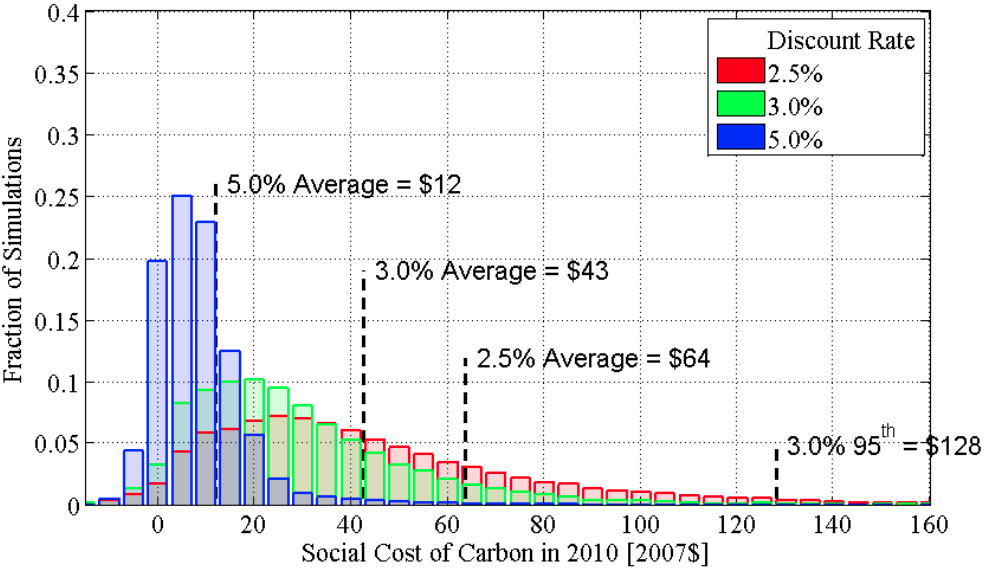
\includegraphics[width=1\textwidth]{scc}
	\caption{Social Cost of Carbon in 2010 (in 2007 dollars per metric ton)}
	\label{USA SCC figure}
\end{figure}

Figure~\ref{USA SCC figure} shows the range of Social Cost of Carbon estimates derived from integrated assessment models.
Despite their sophistication, the results differ by more than an order of magnitude, reflecting underlying value judgments rather than objective consensus.
The utilitarian tradition provides useful insights; it quantifies trade-offs between consumption, savings, and environmental harm, but its reliance on an ideal observer renders it vulnerable to bias.
Each model embeds ethical positions that compete rather than converge, assuming a single planner can prescribe values for all.
Moreover, this framework treats justice as an outcome of arithmetic rather than as a process, overlooking procedural fairness and the plurality of moral worldviews.\\

\begin{quote}
	"Here there are a number of possibilities.
	A collective decision may determine the rate of saving while the direction of investment is left largely to individual firms competing for funds.
	In both a Private Property as well as in a socialist society great concern may be expressed for preventing irreversible damages and for husbanding natural resources and preserving the environment.
	But again either one may do rather badly."~\cite{jr1}
\end{quote}

Critics such as Dasgupta and Sen argue that portraying imperfect economies as though they were initial utopias in this way is a categorical error ~\cite{as1}.
Even among welfare economists, some reject applying pure time preference so that one allows the living to take advantage of their position in time to favour their own interests~\cite{hs1}~\cite{fr1}.
Such examples ignore the possibility for the living to wrong their predecessors or descendants.
Libertarian's might argue that such collective action would lead to violations of individual rights to even a slight extent and therefore should be rejected~\cite{rn1}.
Advocates of the free-market may criticise such methodologies that involve seeking prosperity through centralised long-term coercive planning, rather than appropriate regulation that allows local agents to adjust their activities according to the present situation~\cite{fh1}.
Those of the liberal tradition would consider nothing sacrosanct about the public decision concerning the level of savings and its bias with respect to time preference deserves no special respect~\cite{jr1}.
Consequently, although the Social Cost of Carbon remains an accounting device of sorts, it cannot by itself form a social contract capable of reliably guiding real behaviour.
To find such a tool, we must look beyond aggregate welfare and consider the terms of cooperation under imperfect authority, toward a Hobbesian understanding of the global commons.\\

\subsection{Hobbesian Perspective}

Where utilitarian models seek harmony through aggregated welfare, a Hobbesian perspective begins from a different premise: that harmony itself is precarious.
In Leviathan~\cite{th1}, Hobbes describes order not as the product of shared virtue but as an agreement born from mutual vulnerability.
Individuals surrender certain freedoms in exchange for collective security.
This vision, of imperfect actors cooperating under constraint, makes Hobbes’s logic strikingly relevant to the global commons.
Where no single sovereign authority exists to govern shared resources, yet cooperation remains essential for survival.\\

If the utilitarian question is \emph{"what makes us happiest?"}, the Hobbesian question is \emph{"what keeps us from collapse?2}.
Under such a framework, the cost of maintaining order becomes a measurable proxy for the cost of sustaining life itself.
To capture this relationship, we define the Commonwealth Cost of Carbon (CCC) as a ratio between the resources societies devote to enforcing order and the greenhouse gases they emit.
Greenhouse gas emissions are expected to be a reasonable proxy for overall activity.\\

\begin{equation}
	\frac{anthropogenic\; expenditure\; on\; enforcement}{anthropogenic\; greenhouse\; gas\; emissions}
\end{equation}\\

This expression links moral duty to material accounting.
It estimates how much humanity collectively sacrifices : through defence, policing, and administration, to uphold a life worth living whilst continuing to develop.
It reflects both the economic and ethical costs of sustaining the commons under conditions of imperfect cooperation.\\

As a worked example, we have determined point estimates for the Commonwealth Cost of Carbon in Reporting Years 2000 to 2020.
Greenhouse gas emissions and gross domestic product of each nation-state were collected from the World Banks published World Development Indicators in 2024, consisting of 224 Reporting Nations out of 266 nation-states~\cite{wbank}.
Reported expenditures of nation-states on defense, public order and safety were collected from the International Monetary Fund Data Portal in 2024~\cite{imf}.
Here, it appears Reporting Nations account for ninety eight percent of total global expenditures.
Helpfully, the International Monetary Fund also reports Global gross domestic product.
Global greenhouse gas emissions were inferred for each Reporting Year by dividing Global gross domestic product by the sum of Reporting Nations gross domestic product, before multiplying this ratio by Reporting Nations greenhouse gas emissions.
Global enforcement expenditures were inferred for each Reporting Year by dividing Global gross domestic product by the sum of Reporting Nations gross domestic product, before multiplying the resulting ratio by the sum of Reporting Nations expenditures on defense, public order and safety.\\
A Commonwealth Cost of Carbon has been calculated for each Reporting Year, with the results presented in Figure~\ref{CCC figure}.
Point estimates for the Commonwealth Cost of Carbon in current prices are ~2020\$140tCO2e, up from ~2000\$65tCO2e.
The figure appears to demonstrate a trend of degrading ecosystem performance over the Reporting Years.
Such insight appears to suggest the action to save greenhouse gas emissions have become more valuable.\\

\begin{figure}[H]
\centering
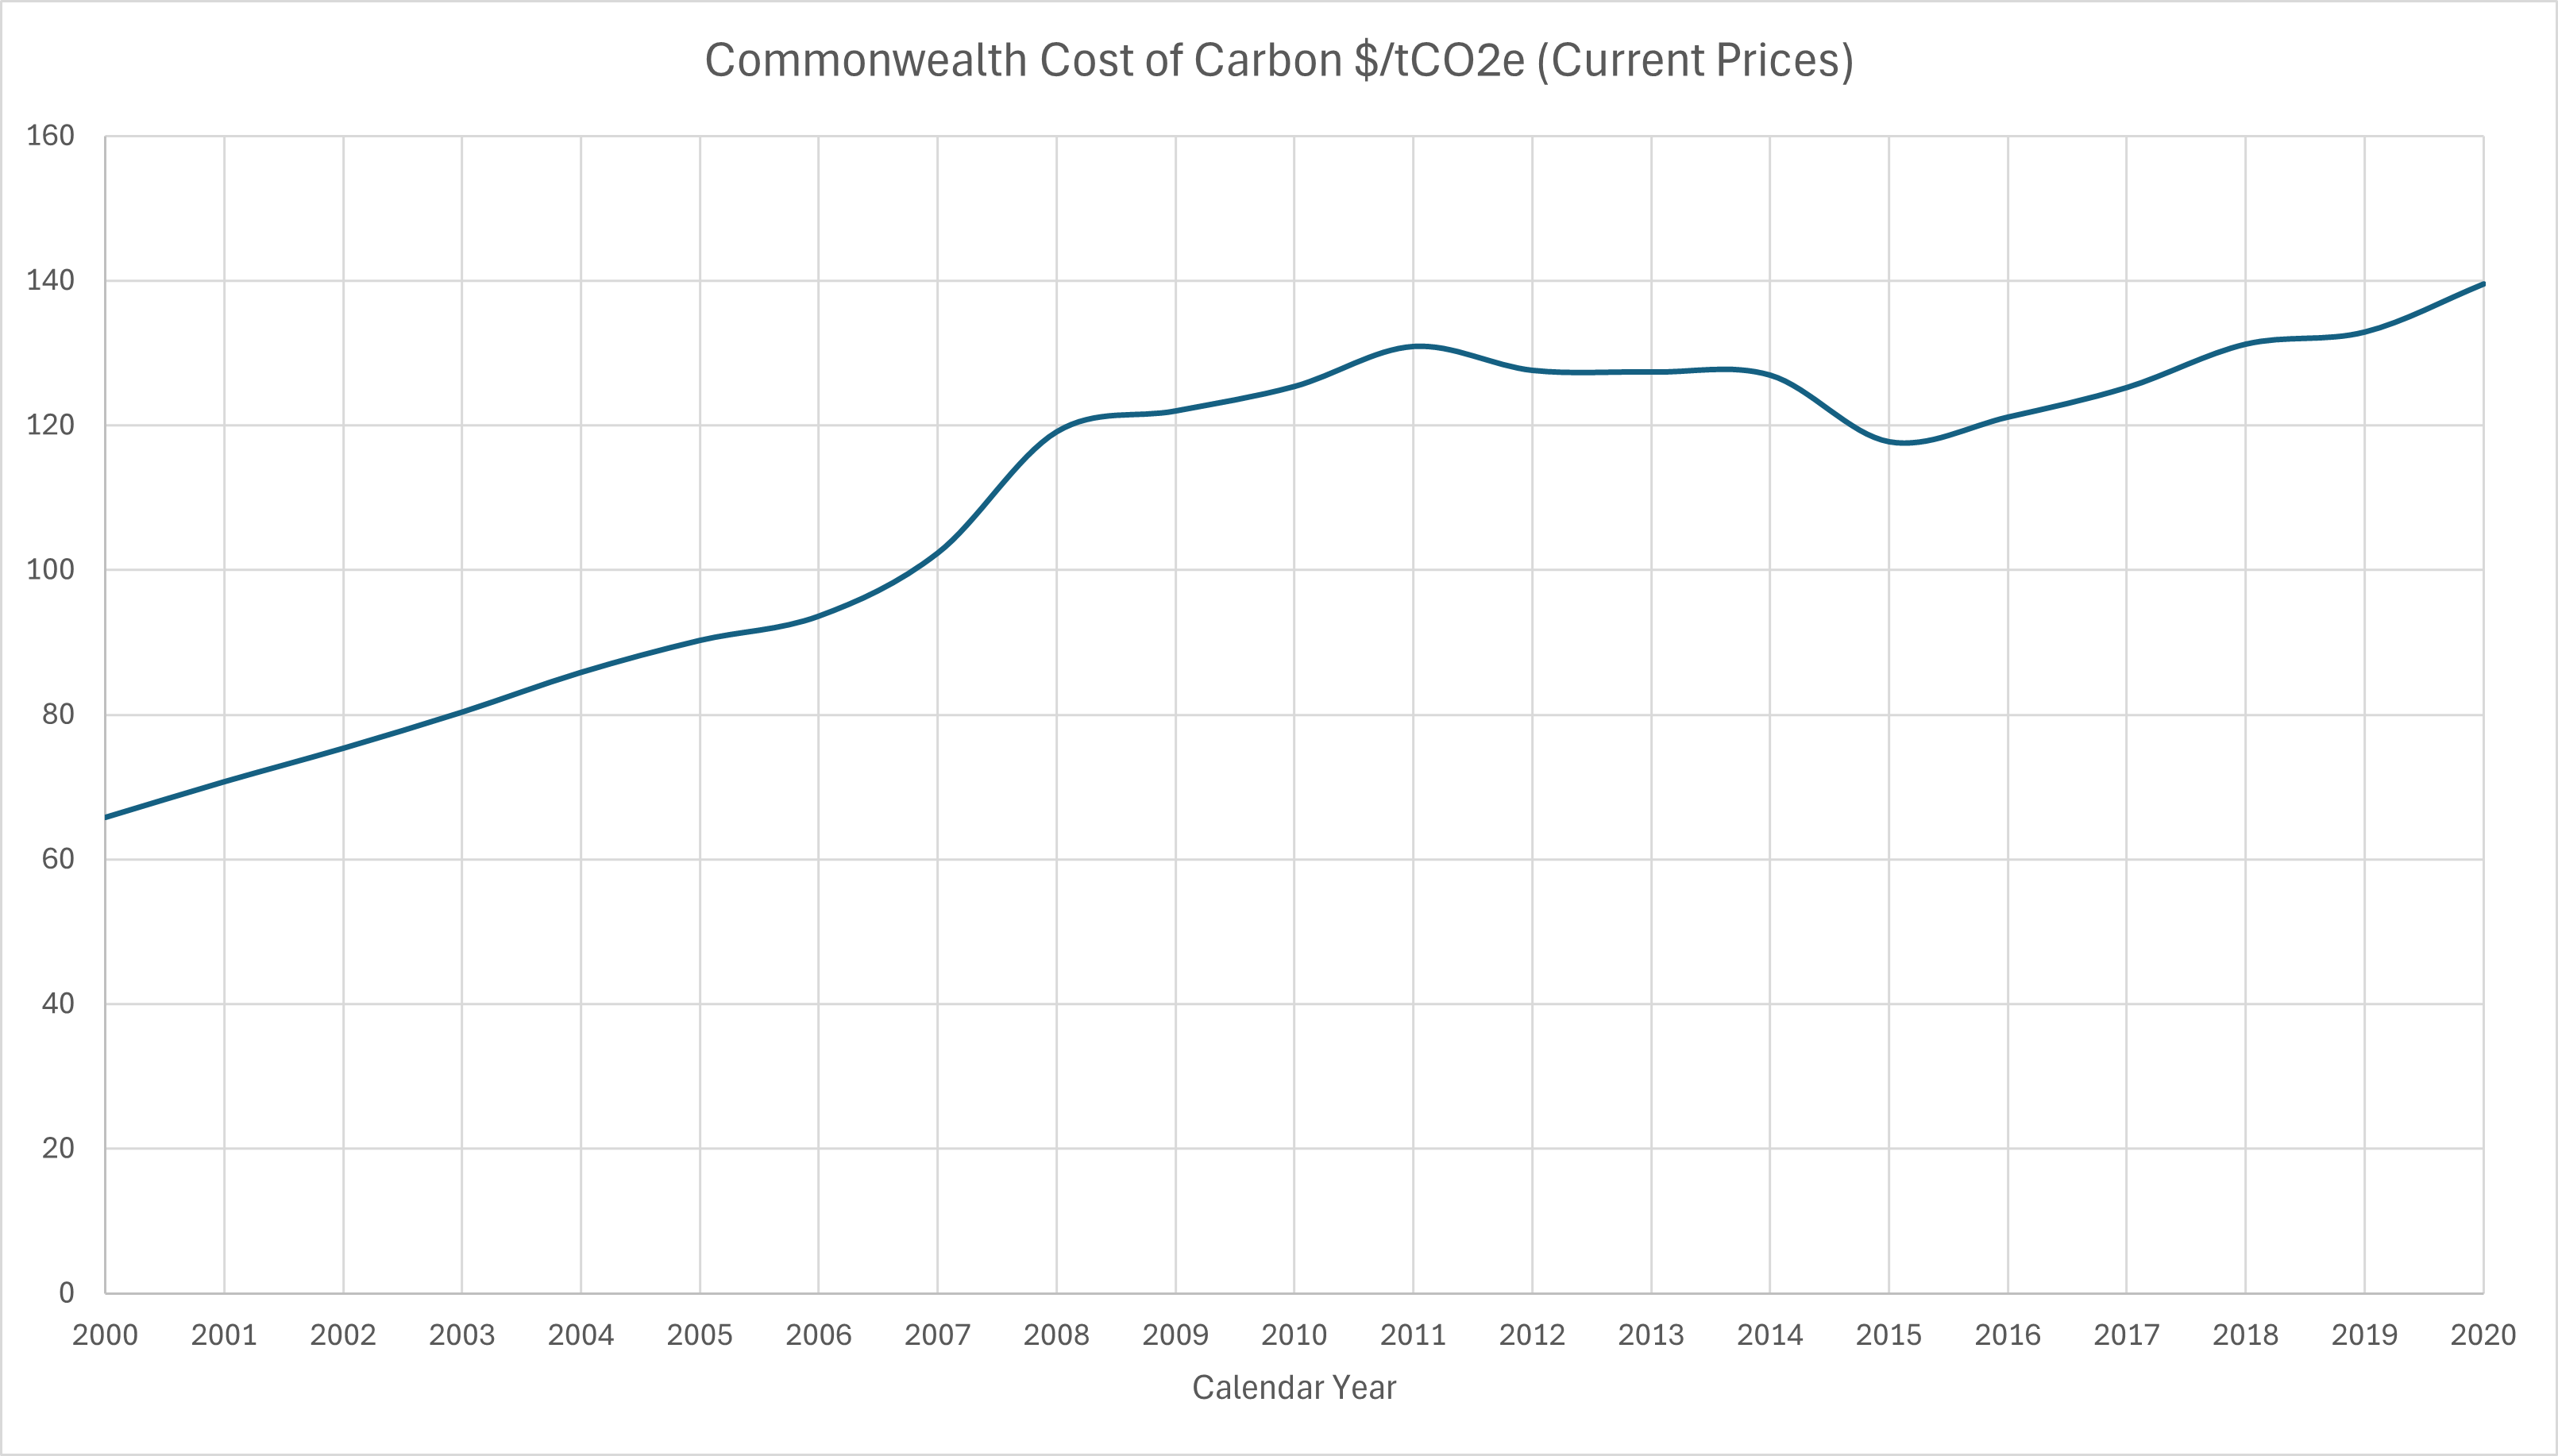
\includegraphics[width=1\textwidth]{ccc}
\caption{Commonwealth Cost of Carbon \$tCO2e (current prices)}
\label{CCC figure}
\end{figure}

The indicator’s simplicity is its strength: anyone can compute it using open data, without recourse to expert integrated assessment models or privileged knowledge.
It therefore serves not only as a quantitative measure but also as a moral statement.
A transparent accounting of how much societies pay, in the broadest sense, to sustain living conditions within natural disorder.
Hobbes would likely interpret this ratio as evidence that coercive structures, laws, enforcement, and collective sanctions remain indispensable, even when penalties are rarely exercised.
Without such machinery, he warned, humanity would risk \emph{"a war of every man against every man"}.
In our context, the CCC quantifies the ongoing sacrifice that prevents such collapse, the expenditure that buys historic stability.
Carbon emissions thus appear not only as pollutants but as signatures of human interdependence; their true cost includes the price of sustaining peace.
Philosophically, the Commonwealth Cost of Carbon reinterprets environmental economics through the lens of the social contract.
It does not presume altruism, nor rely on an omniscient planner.
Instead, it measures cooperation under constraint: how much order we purchase in service to a life worth living.
By doing so, it translates Hobbes’s seventeenth-century insight into a twenty-first-century metric.
An auditable measure of ecosystem performance that reveals whether our collective expenditures remain commensurate with the stability we claim to value.\\

\section{Strategic Planning}  **RE-WRITE FROM HERE**

This research has established a global ecosystem performance indicator applicable to ones entire history.
Such insights provide the opportunity to embed long-term strategy for sustainable action.
When applying the Commonwealth Cost of Carbon in addition to John Rawls Principles of a Society of Peoples, one arrives at an original constitution of a \emph{Commonwealth of Peoples}.
At this point the constitution of the Commonwealth of Peoples is considered comprehensive philisophical doctrine, both a stable and protected belief.
One is also mindful of the possibility that some may find spiritual connections with any indicator that measures a societies sacrifice to maintain the status quo.
The Commonwealth Cost of Carbon appears an instrument that requires some respect.
Although, the Commonwealth of Peoples is established as an inter-networking or inter-faith guild that offers nothing to necessarily worship in itself.\\

Our constitution is not enough to promote wider engagement and action.
It is our proposition that some sort of vision, hypothesis or prospect is needed for a shared understanding.
We recognise that small changes to the quality of services can have significant impacts on requirements for supply infrastructure.
Realising infrastucture savings could be a more fruitful activity than simply making radical changes to the quality of infrastructure provided.
Therefore, the management of service quality appears a strong candidate for action.
How can a Commonwealth Cost of Carbon be used to inform service performance marketing?\\

An exercise in strategic planning from our newly identified position was initiated.
Parkinson et al. outlines a useful taxonomy of methods for scenario planning, which may be used~\cite{atp1}.
Whilst it is tempting here to use the Commonwealth Cost of Carbon in financial forecasts for future generations, we are more concerned with the present.
An exercise of prospective scenario planning is a recognised methodology to explore qualitative possibilities for developing longer term plans.
Such techniques consider what could conceivably happen, rather than determining probable or preferred outcomes.\\

As this initiative was something of an outcast, we did not the opportunity to engage a wider group of peers.
It would have been preferrable at this stage to include a large workshop of experts within this exercise.
Therefore, ones scenario planning has been undertaken by the authors alone.\\

Initially, this research set out to establish two driving forces.
It is believed that one of these driving forces involved the magnitude of the service, represented by service cost.
One also determined that another driving force required a \emph{"Service Rating"} representative of the quality of service greenhouse gas emissions.
Such a Service Rating can be used to compare the performance of services on a consistent basis anywhere worldwide.
One applied the following equation to establish Service Rating for a consistent period of time, which is conceived as a simple cost-benefit ratio.\\

\begin{equation}
	\frac{C  \cdot \;Commonwealth\; Cost\; of\; Carbon\;}{service\; cost\;}
\end{equation}

Where, $C$ is greenhouse gas emissions of service from source to end-use.
One believes it is not allowable for this value to be adjusted in any way through investments in other services, such as national grid connected renewable generation of electricity.
There is an importance associated with considering the services in a configuration that can be witnessed \emph{"as-is"}.\\

As a result, the following prospective scenarios were arrived at for service performance marketing.
These scenarios consider individual end-states and represent grounds for a common-sense hypothesis or prospect.
Such insights seem to be only testable through action research and represent ones point of departure from theory.
We do not consider any of these scenario end-states as favourable to another, as they are actually inter-dependent and co-existing.
Whilst sites with a higher Service Rating may be less habitable, this does not make such a case any less rewarding.
The scenarios simply illustrate the different professions that may take priority in making efforts towards sustainable ecosystems.
Such projections could prove useful in introducing professional services to property owners.
It is our expectation that a combination of service quality and service magnitude will dictate which professional service take priority.
Figure~\ref{Scenarios} illustrates the types of services that may be prioritised at plausible service limits.
Whilst Table~\ref{Service limits table} suggests possible site typologies to be serviced at these limits.\\

\begin{figure}[H]
\centering
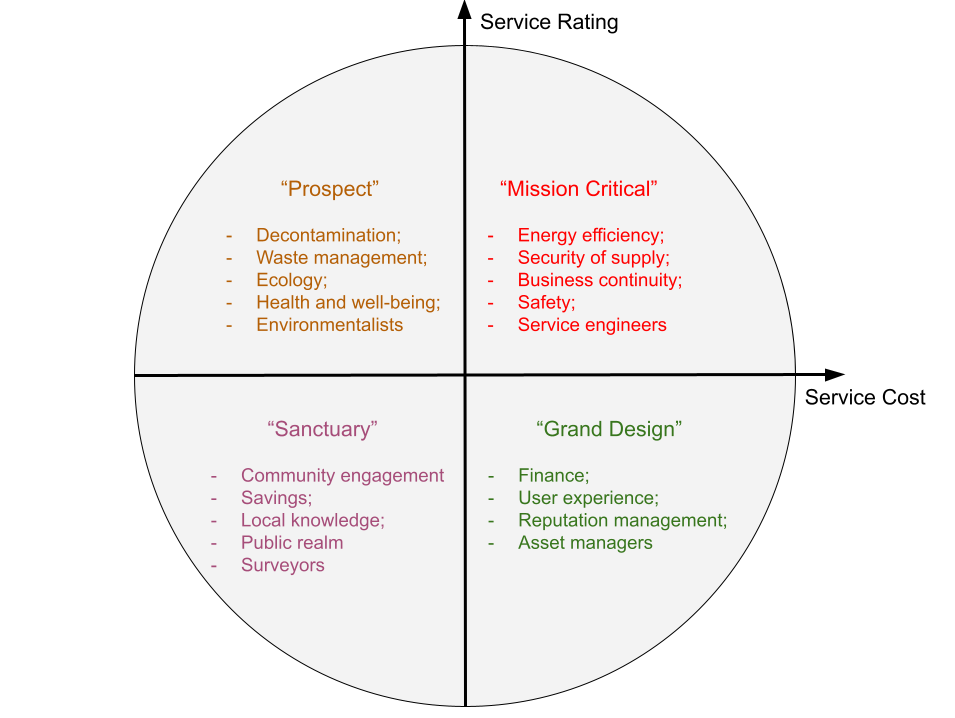
\includegraphics[width=1\textwidth]{scenarios}
\caption{Scenarios for Service Performance Marketing}
\label{Scenarios}
\end{figure}

\begin{table}[H]
\caption{Possible Site Typologies at Plausible Service Limits}
\begin{center}
\begin{tabular}{| l | l |}
\hline
Service Performance Scenario&Site Typology\\
\hline
Prospect&Landfill\\
Sanctuary&Tent\\
Mission Critical&Data Centre\\
Grand Design&Golf Club\\
\hline
\end{tabular}
\end{center}
\label{Service limits table}
\end{table}

Believing ones narrative to be reasonable, consideration is made towards selecting technologies for implementation.
Stable agreements of Ecosystem Performance and Service Rating may be made between any legal entities, including individuals and organisations.
Such agreements could be supported by distributed peer-to-peer blockchain, with peer endorsement of Ecosystem Performance and Service Rating transactions.
These transactions would be formed of standard contracts, defined in chaincode.
This could result in a fully auditable and assured enterprise grade root source of trust to enable secure transactions worldwide.\\

\section{Conclusions}

This research asks how societies can coordinate fairly when nation-states alone cannot manage the global commons.
It has been observed that it is implausible to consider a society entirely free of Realpolitik.
Therefore, societies continue to be subjected to a social cost that necessitates service.
As a result we regard propositions of ideal societies, such as John Rawls Society of Peoples, an incomplete thesis for practice.\\

Our research has developed the Commonwealth Cost of Carbon as a novel Ecosystem Performance Observation.
It is derived through a simple formula that does not require scientific expertise to calculate and is relatively simple to audit.
Point estimates for the Commonwealth Cost of Carbon in current prices are ~\$140tCO2e in 2020, up from ~\$65tCO2e in 2000.
This appears to demonstrate a trend of degrading ecosystem performance.
Such insight appears to suggest the action to save greenhouse gas emissions have become more valuable.
This indicator has many advantages over notable precendents that estimated social costs of carbon, which required privilaged access to an ideal observers development plans.
Anyone could find the legitimacy, means and ability to calculate a Commonwealth Cost of Carbon for themselves before deciding whether to agree.\\

When applying the Commonwealth Cost of Carbon together with John Rawls Principles of a Society of Peoples a new guild is constituted.
We have initiated this guild as the Commonwealth of Peoples.
To improve engagement and develop a shared understanding for action, a novel indicator of service quality has been proposed.
This Service Rating is a basic cost-benefit ratio.
We believe this Service Rating indicator can be used together with service magnitude as a service performance marketing axis that prioritises professional services offered to property owners.
Through this mechanism, the Commonwealth of Peoples can become a tool for practical action.\\

In conclusion, we believe the Commonwealth of Peoples has distinct advantages over nation-states approaches to managing the global commons.
We claim a grounding in comprehensive philsophical doctrine, rather than privilaged Realpolitik.
No projections have been made over future generations.
Our accounts may be shared in common with all and do not require expert judgement.
Beyond reasonable doubt, the Commonwealth of Peoples is now prepared for application to the present generation.\\

\begin{thebibliography}{99}

\bibitem{jr2} Rawls~J. (1999)
\emph{The Law of Peoples}
Cambridge, MA and London: Harvard University Press

\bibitem{jl1} Locke~J. (1967)
\emph{Two Treatises of Government}
Cambridge: Cambridge University Press
	
\bibitem{rn1} Nozick~R. (1974)
\emph{Anarchy, State and Utopia}
New York, NY: Basic Books
	
\bibitem{th1} Hobbes~T. (1668)
\emph{Leviathan},
Oxford: Oxford University Press

\bibitem{rc1} Coase~R.H. (1960)
\emph{The Problem of Social Cost.},
The Journal of Law and Economics, 3, pp. 1-44

\bibitem{pd3} Dasgupta~P. (2015)
\emph{Disregarded Capitals: What National Accounting Ignores.},
Accounting and Business Research, 45(4), pp. 122-138

\bibitem{hs1} Sidgwick~H. (1877)
\emph{The Methods of Ethics}
Cambridge: Cambridge University Press

\bibitem{pd2} Dasgupta~P. (2001)
\emph{Valuing Goods.},
In: Human Well-Being and the Natural Environment. Oxford: Oxford University Press, pp. 122-138

\bibitem{ka1} Arrow~K.J. (1963)
\emph{Social Choice and Individual Values},
New York, NY: John Wiley
	
\bibitem{km1} May~K. (1952)
\emph{A Set of Necessary and Sufficient Conditions for Simple Majority Decisions},
Econometrica, 20(4), pp. 680-684

\bibitem{as2} Sen~A. (1970)
\emph{Collective Choice and Social Welfare}
San Francisco: Hoden Day

\bibitem{jw2} Waldron~J. (1984)
\emph{Theories of Rights}
Oxford: Oxford University Press
		
\bibitem{rd1} Dworkin~R. (1978)
\emph{Taking Rights Seriously}
London: Duckworth

\bibitem{fr1} Ramsey~F.P. (1928)
\emph{A Mathematical Theory of Saving.}
Economic Journal, 38(152) pp. 543-559

\bibitem{wc1} Cline~W.R. (1992)
\emph{The Economics of Global Warming},
Washington D.C.: Institute for International Economics
		
\bibitem{wn1} Nordhaus~W.D. (1994)
\emph{Managing the Global Commons: The Economics of Climate Change},
Cambridge, MA: MIT Press
	
\bibitem{ns1} Stern~N.H. (2006)
\emph{The Stern Review of the Economics of Climate Change},
Cambridge: Cambridge University Press
		
\bibitem{ch1} Hope~C., Anderson~J., Wenman~P. (1993)
\emph{Policy Analysis of the Greenhouse Effect. An Application of the PAGE Model},
Energy Policy, 21, pp. 327-338
		
\bibitem{rsjt1} Tol~R.S.J. (1997)
\emph{On the Optimal Control of Carbon Dioxide Emissions: An Application of FUND},
Environmental Modelling and Assessment, 2, pp151-163

\bibitem{iwg1} Interagency Working Group on Social Cost of Carbon, United States Government (2013)
\emph{Technical Support Document: - Technical Update of the Social Cost of Carbon regulatory Impact Analysis - Under Executive Order 12866},
Washington D.C.: United States Government

\bibitem{jr1} Rawls~J. (1971)
\emph{A Theory of Justice}
Cambridge, MA and London: Harvard University Press

\bibitem{as1} Sen~A. (1961)
\emph{On Optimizing the Rate of Saving}
Economic Journal, 71
		
\bibitem{ms1} Marglin~S.A. (1961)
\emph{The Social Rate of Discount and The Optimal Rate of Investment}
The Quaterly Review of Economics, 77(1), pp. 95-111

\bibitem{fh1} Hayek~F. (1944)
\emph{The Road to Serfdom}
Chicago: University of Chicago Press

\bibitem{wbank} World Bank (2024)
\emph{World Development Indicators}
Accessed 13/11/2024, available online: 
\url{https://databank.worldbank.org/source/2?country=IRN&l=en}

\bibitem{imf} International Monetary Fund (2024)
\emph{IMF Data}
Accessed 13/11/2024, available online: 
\url{https://data.imf.org/en}

\bibitem{atp1} Parkinson~A.T., Friedman~K.S., Hacking T., Guthrie~P.M. (2012)
\emph{Exploring Scenarios for the Future of Energy Management in Property.},
Building Research and Information, 40(3), pp. 373-388
	
\end{thebibliography}



\end{document}